\section{Practical Case}\label{s:practical_case}
To demonstrate the usage of the Moment Generating Function for computing moments of fractional order, we consider a dataset containing the weekly S\&P 500 index from the second week of January 2000 up until the last week of December 2024, provided by Wharton Research Data Services.
\subsection{First look at the data}
 The following figure depicts the trend of the S\&P 500 index over time:

\begin{figure}[H]
    \centering
    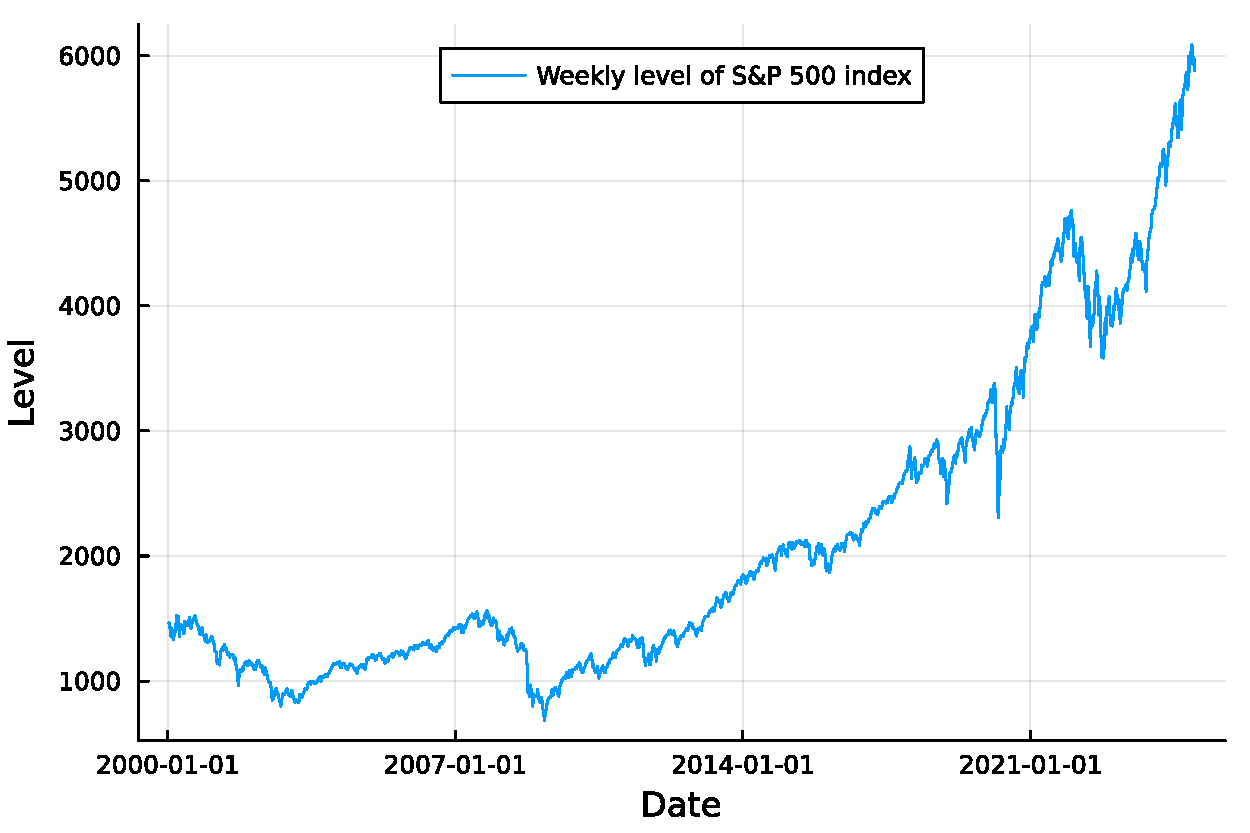
\includegraphics[width=0.7\textwidth]{figures/stock_level.pdf}
    \caption{S\&P 500 level over time}
    \label{fig:stock_level}
\end{figure}
It is clear from figure \ref{fig:stock_level} that the S\&P 500 index is non-stationary, as the mean of the process is not constant. We prefer to work with data that is stationary, thus we consider the log-returns (variations in stock-price) as shown in figure \ref{fig:stock_returns}. These values have been scaled by a factor of 100 to express them as percentages

\begin{figure}[H]
    \centering
    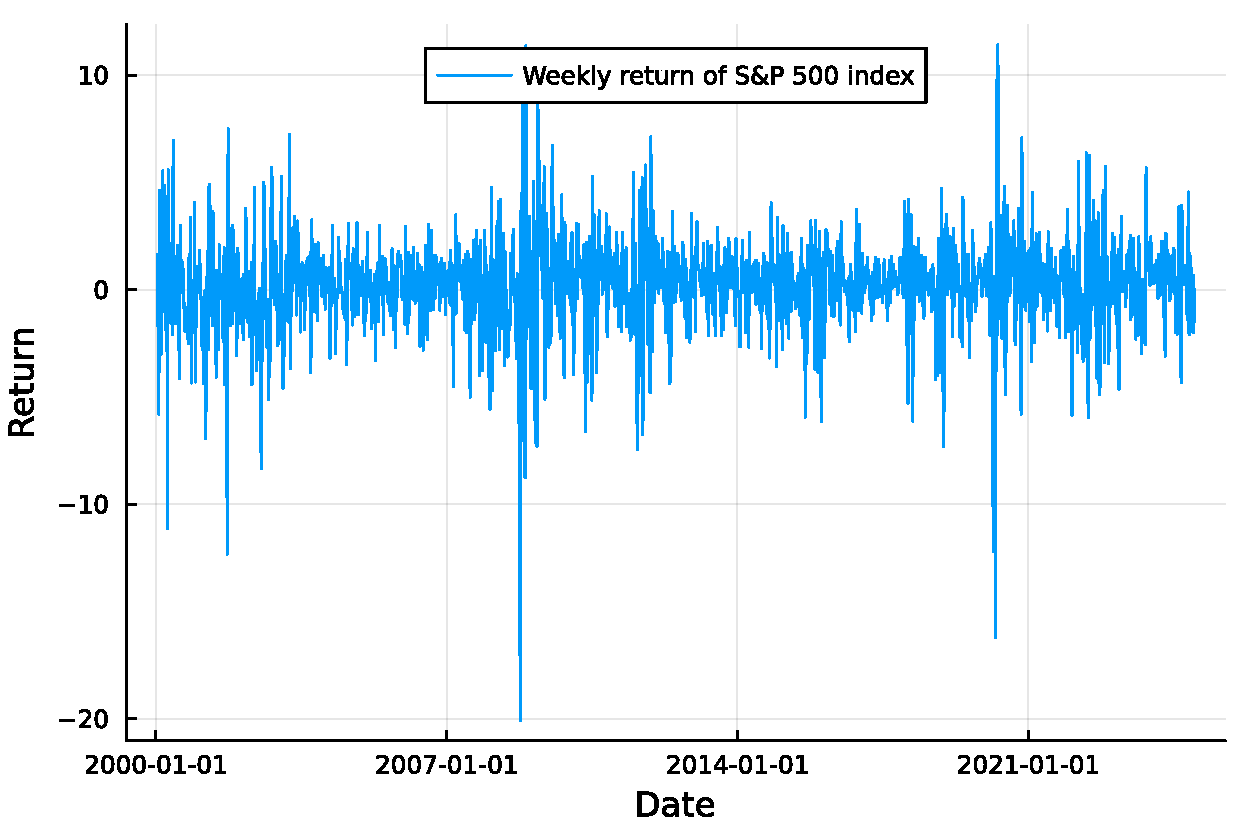
\includegraphics[width=0.7\textwidth]{figures/stock_returns.pdf}
    \caption{S\&P 500 log-returns over time}
    \label{fig:stock_returns}
\end{figure}
The log-returns series appears more suitable for volatility analysis compared to the data displayed in figure \ref{fig:stock_level}. The mean of the log-returns seems to be stationary (lying around zero), the variance of the log-returns also seems to remain constant over time. Additionally, there are no signs of seasonality. Notable spikes in the log-returns around 2008 and 2021 likely correspond the global financial crisis and COVID pandemic respectively. In times of (financial) uncertainty, it is more likely that returns may take more extreme values, making them less predictable.
\newline

The following core statistics of the log-returns, as displayed in figure \ref{fig:stock_returns} have been computed:

\begin{table}[H]
    \centering
\begin{tabular}{ccccc}
  \toprule
  \textbf{Mean} & \textbf{Variance} & \textbf{Skewness} & \textbf{Kurtosis} & \textbf{P-value}\\\midrule
  0.108 & 6.17 & -0.878 & 7.225 & 1e-99 \\\bottomrule
\end{tabular}

\caption{Summary Statistics log-returns of S\&P 500} 
\label{tab:summary_statistics}
\end{table}
Indeed, as anticipated, the (unconditional) mean seems to be around zero. Moreover, the rather great value of the kurtosis in table \ref{tab:summary_statistics} indicates that the log-returns of the S\&P 500 are not normally distributed, as this value is far greater than 3 which is expected in the context of financial markets, due to frequent occurrence of extreme values. The normal distribution, known for its thin tails, underestimates the probability of such extremes. The p-value included in table \ref{tab:summary_statistics} is the associated p-value of the augmented Dickey-Fuller unit root test, with null hypothesis: the log-returns of the s\&P 500 stock index is a unit root process.  The p-value is so small that we reject the hypothesis at any conventional significance level. Thus, we can formally conclude that the weekly log-returns of the S\&P 500 index are stationary.

\subsection{Modelling volatility of the log-returns}
It is well known that the stock prices, as well as the mean of log-returns, cannot be predicted. Therefore, we focus on the volatility of the log-returns instead. A widely used approach is the autoregressive conditional heteroskedasticity model of order \(q\), denoted ARCH(q), introduced by \cite{engle1982}. With observation equation: 
\begin{equation}
    r_t = \sigma_t \cdot \epsilon_t
\end{equation}

and updating equation:

\begin{equation}
    \sigma^2_t = \omega + \sum_{i = 1}^{q} \alpha_i \cdot r^2_{t-i}
\end{equation}

Another commonly used model is the Generalized Conditional Heteroskedasticity model of order \((p, q)\), denoted GARCH(p, q), as proposed by \cite{bollerslev1986} with observation equation

\begin{equation}
    r_t = \sigma_t \cdot \epsilon_t 
\end{equation}

and updating equation:

\begin{equation}
    \sigma^2_t = \omega + \sum_{i = 1}^{p} \beta_i \cdot \sigma^2_{t-i} + \sum_{i = 1}^{q} \alpha_i \cdot r^2_{t-i}
\end{equation}
To determine which model is more appropriate for monitoring volatility, we first examine the autocorrelation function (ACF) of the data. The ACF of log-returns is typically close to zero, and is therefore considered to be negligible in practice. Instead, we analyse the autocorrelation function of the squared log-returns.
The following figure depicts the autocorrelation function of the squared log-returns (note that the first index at \(t = 0\) has been removed as \(corr(r_i, r_j)\) is always equal to 1 for \(i = j\)).

\begin{figure}[H]
    \centering
    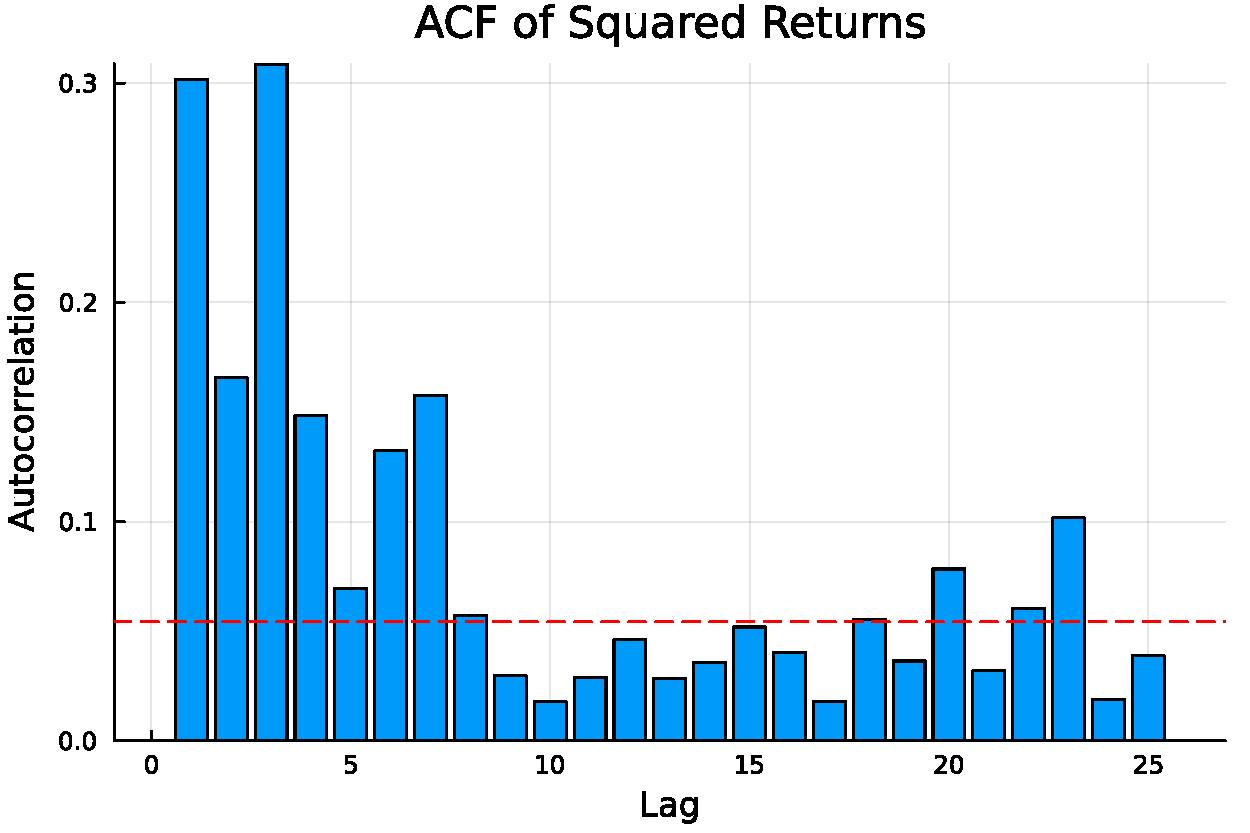
\includegraphics[width=0.7\textwidth]{figures/acf_squared_returns.pdf}
    \caption{ACF of Squared log-returns}
    \label{fig:acf_squared_returns}
\end{figure}

From figure \ref{fig:acf_squared_returns} we observe that a substantial number of lags exhibit autocorrelations exceeding the 95\% confidence interval (given by the red dashed line). This suggests that autocorrelation function does not decay exponentially and that an ARCH(1) model would be inadequate for describing the volatility in this dataset. Consequently, we GARCH\((p, q)\) model. We opt for the latter, as choosing the former often leads to too many parameters to estimate.

To determine the number of parameters \(p\) and \(q\) such that the GARCH\((p,q)\) model describes the volatility of the data the best, we compute the Akaike information criterion (AIC) and the Bayesian information criterion (BIC). The model having both the lowest AIC and BIC value is to be preferred. We consider GARCH\((p, q)\) models for \(p, q \in \{1, 2, 3\}\).

\begin{table}[H]
    \centering
\begin{tabular}{ccc}
  \toprule
  \textbf{Model} & \textbf{AIC} & \textbf{BIC} \\\midrule
  GARCH(1,1) & 5699 & 5714 \\
  GARCH(1,2) & 5700 & 5721 \\
  GARCH(1,3) & 5697 & 5723 \\
  GARCH(2,1) & 5700 & 5721 \\
  GARCH(2,2) & 5702 & 5728 \\
  GARCH(2,3) & 5699 & 5730 \\
  GARCH(3,1) & 5702 & 5727 \\
  GARCH(3,2) & 5703 & 5734 \\
  GARCH(3,3) & 5699 & 5735 \\\bottomrule
\end{tabular}

\caption{AIC and BIC for GARCH models} 
\label{tab:aic_bic}
\end{table}

From table \ref{tab:aic_bic} we observe that the GARCH(\(1, 3\)) model achieves the lowest AIC value, while the GARCH(\(1, 1\)) has the lowest BIC value. Both models also obtain relatively low values for the other criterion, indicating that they are good candidates for modeling volatility. For simplicity, we proceed with the GARCH\((1, 1)\) model as that means we will only need to estimate three parameters instead of five, leading to more straightforward interpretability.

The parameters have been estimated using Maximum Likelihood Estimation. Link functions were applied to ensure non-negativity of the parameters and that the log-returns form a weakly stationary white noise process.

\begin{table}[H]
    \centering
\begin{tabular}{ccc}
  \toprule
  \textbf{Parameter} & \textbf{Estimate} & \textbf{Standard error} \\\midrule
  \(\omega\) & 0.37 & 0.084 \\
  \(\alpha\) & 0.224 & 0.030 \\
  \(\beta\) & 0.726 & 0.031 \\\bottomrule
\end{tabular}

\caption{Parameter Estimates of GARCH(1,1)} 
\label{tab:parameter_estimates}
\end{table}

Indeed, \(\hat{\alpha} + \hat{\beta} < 1\) confirming that the log-returns represent a weakly stationary white noise sequence. Moreover, the standard errors of the estimates are relatively small, indicating high precision.


\subsection{Using fractional moments to analyse the log-returns}
Now that we have described the data using core statistics, fitted appropriate models and estimated their parameters, we finally consider the usage of moments of fractional order to enhance the analysis.
\subsubsection{Computing conditional absolute moments of fractional order}\label{sssec:conditional_fractional_moments}
Following \cite{hansen2024}, we compute the conditional expectation of the absolute variance over a given period \(H\), specifically
\[\mathbb{E}[|X_{T + H}|^\gamma \mid \mathcal{F_T}],\]
 where \(X_{T+H} = Var(R_{T, H}) = \mathbb{E}[R_{T, H}^2] = \mathbb{E}[\sum_{t = T + 1}^{T + H} r_t^2] = \sum_{t = T + 1}^{T + H}\mathbb{E}[ r_t^2] \). Here \(r_t\) denotes the log-return at time \(t\) and \(\mathcal{F_T}\) represents the natural filtration, which is the sigma-algebra generated by the process up to time \(T\) \cite{lowther2009}. In other words, \(\mathcal{F_T}\) contains all information about log-returns observed up to time \(T\). Note that \(Var(R_{T, H})\) is indeed equal to \(\mathbb{E}[R_{T, H}^2]\) as \(\mathbb{E}[R_{T, H}]^2 = \mathbb{E}[\sum_{t = T + 1}^{T + H} r_t]^2 = \left(\sum_{t = T + 1}^{T + H} \mathbb{E}[r_t]\right)^2\). We assume that \(r_t \sim \mathcal{N}(0, \sigma^2_t)\) and since the autocorrelation function of log-returns is zero, we have that each \(r_t\) is independent of the observations at different time indices. So it follows that: \(\left(\sum_{t = T + 1}^{T + H} \mathbb{E}[r_t]\right)^2 = \left(\sum_{t = T + 1}^{T + H} 0\right)^2 = 0\). To avoid confusion, we denote the order of the fractional moment by \(\gamma\) rather  than \(\alpha\) which is already used as a parameter in the GARCH(1,1) model. We compute moments of order \(\gamma \in \{-0.5, 0.5, 1.5, 2\}\) as suggested by \cite{hansen2024}.
According to \cite{hansen2024} the orders of \(\gamma\) correspond to the following moments:

\begin{itemize}
\item \(\gamma = -0.5\): Inverse of the volatility of the returns. May be used for Sharpe ratio forecasting
\item \(\gamma = 0.5\): Conditional volatility or standard deviation of  returns
\item  \(\gamma = 1.5\): Conditional skewness (of the absolute value)
\item  \(\gamma = 2\): Conditional kurtosis
\end{itemize}

These fractional methods are computed using three different methods. 
\begin{itemize}
\item \textbf{Empirical Simulation: } We consider the empirical value of the moments, obtained by performing 100.000 Monte Carlo simulations of the distribution of the variance (see algorithm \ref{alg:simulate_conditional_variance}) followed by averaging the results to obtain the empirical estimates.
\item \textbf{Integral method: } We compute the standard integral, namely \(\int_{-\infty}^{\infty} (x)^\gamma f_X(x) \, dx\), where \(f_X(x)\) is the PDF of \(X_{T,H}\). This PDF is acquired by performing Kernel Density Estimation on the values of \(X_{T,H}\).
\item \textbf{Caputo-Fabrizio MGF: } We also compute the expectations of fractional order using the inaccurate method of the Caputo-Fabrizio MGF. This integral also makes use of the same PDF obtained by Kernel Density Estimation.
\end{itemize} 

We compute these moments for different time horizons, namely \(H \in \{4, 8, 16\}\). That is, we compute the expectation of the absolute variance of order \(\gamma\) for one month, two months and four months in the future, respectively. This allows us to evaluate whether the time horizon affects the performance of the Caputo-Fabrizio method. The full procedure is detailed in algorithm \ref{alg:analyse_fractional_moments}.

We obtain the following table:


\begin{table}[H]
    \centering
\begin{tabular}{ccccc}
  \toprule
  \textbf{H} & \textbf{order} & \textbf{empirical} & \textbf{standard} & \textbf{CF} \\\midrule
  4 & -0.5 & 0.25 & 0.255 & 0.138 \\
  4 & 0.5 & 4.948 & 4.938 & 1.855 \\
  4 & 1.5 & 201.653 & 201.763 & 56.748 \\
  4 & 2.0 & 1568.7 & 1569.69 & 1569.69 \\
  8 & -0.5 & 0.164 & 0.164 & 0.06 \\
  8 & 0.5 & 7.098 & 7.095 & 1.94 \\
  8 & 1.5 & 552.323 & 552.142 & 114.85 \\
  8 & 2.0 & 5909.13 & 5905.96 & 5905.96 \\
  16 & -0.5 & 0.113 & 0.113 & 0.028 \\
  16 & 0.5 & 10.073 & 10.066 & 1.971 \\
  16 & 1.5 & 1550.63 & 1547.5 & 230.747 \\
  16 & 2.0 & 23559.0 & 23482.6 & 23482.6 \\\bottomrule
\end{tabular}

\caption{Conditional expectations for various orders} 
\label{tab:conditional_expectations}
\end{table}
The results from table \ref{tab:conditional_expectations} can be interpreted as follows:

\begin{itemize}
\item \(\gamma = -0.5\): The inverse of the volatility decreases with \(H\), implying that the volatility increases as the forecast horizon extends. All values are positive, due to use of absolute moments.
\item \(\gamma = 0.5\): The standard deviation of the returns indeed increase when the value of \(H\) increases. This is expected as greater time horizons lead to more uncertainty.

\item  \(\gamma = 1.5\): The conditional skewness greatly increases when the value of \(H\) increases. However, since we examine the absolute value, all skewness values are positive, making the interpretability limited.

\item  \(\gamma = 2\): The conditional kurtosis vastly increases as the value of \(H\) increases. For all values of \(H\), the kurtosis is considerably greater than 3, implying that the conditional absolute cumulative returns are not normally distributed. As with skewness, the interpretability is limited due to the use of absolute values.
\end{itemize}

For all values of \(H\) and non-integer values of \(\gamma\) the empirical results and  theoretical  integral results are closely aligned. Similarly, for all values of \(H\) and \(\gamma = 2\), the results of the integral method and Caputo-Fabrizio MGF are the same, as the latter is accurate for integer derivatives of the MGF. As indicated in section \ref{s:simulation}, the Caputo-Fabrizio MGF greatly under-estimates the values of fractional moments. These errors increase with \(H\), implying that the method increasingly underestimates volatility - and hence risk - for longer horizons. We therefore conclude that the Caputo-Fabrizio MGF is unreliable for computing expectations of fractional order in forecasting applications. This conclusion is consistent with the results of section \ref{ss:accuracy_analysis}, where the size of the errors grew as the distribution parameters increased. Figure \ref{fig:conditional_moments_error} emphasizes the increment of the errors of the Caputo-Fabrizio MGF.



\begin{figure}[H]
    \centering
    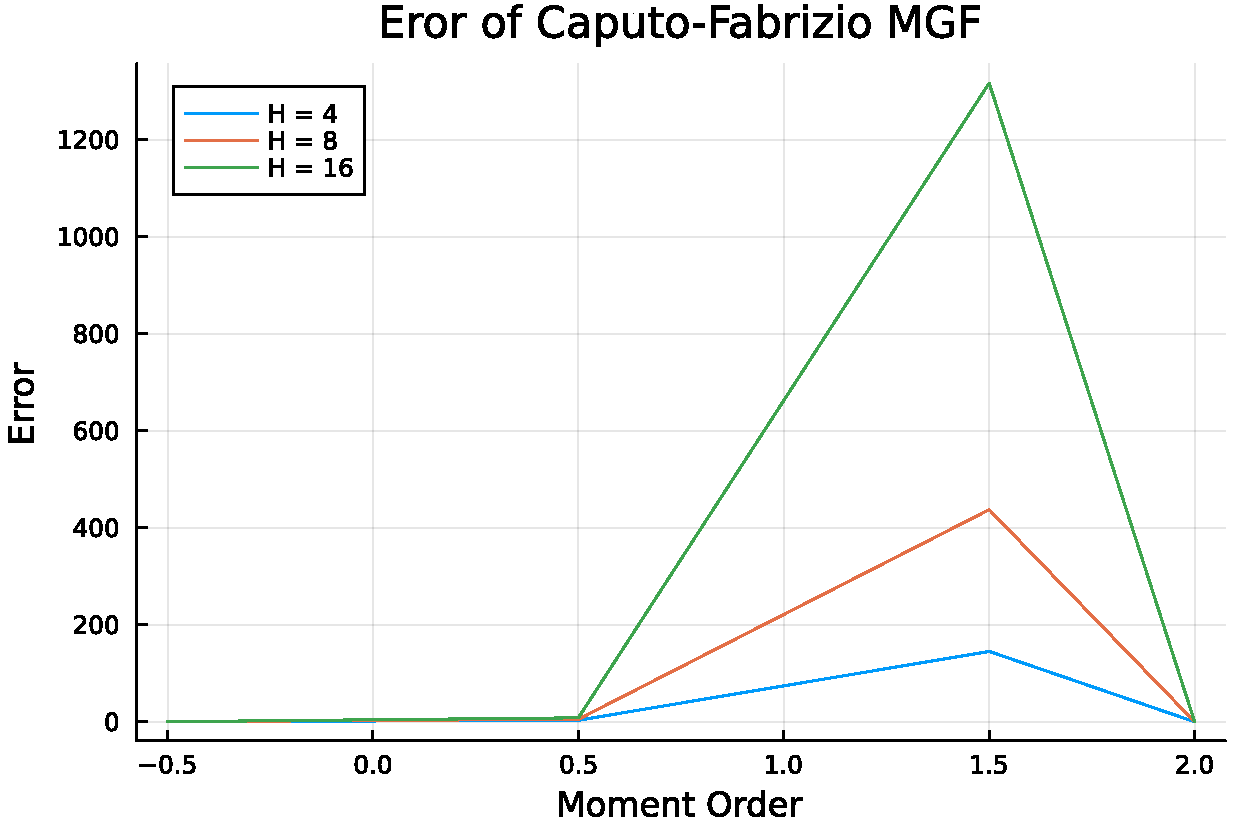
\includegraphics[width=0.7\textwidth]{figures/conditional_moments_error.pdf}
    \caption{Error of Caputo-Fabrizio MGF for various values of \(H\) and \(\gamma\)}
    \label{fig:conditional_moments_error}
\end{figure}\

Note that figure \ref{fig:conditional_moments_error} only includes discrete values of \(\gamma \in \{-0.5, 0.5, 1.5, 2\}\). Therefore, the plotted functions may give a misleading impression of continuity. For instance, the error at \(\gamma = 1\) should be exactly zero, yet the graph figure suggests otherwise due to the interpolation between points.

\subsubsection{More about the computation and interpretability of fractional moments}
An observant reader might wonder why we compute the expectation of \(| X_{T + H}|\) instead of simply computing the expectation of \( X_{T + H}\). We have that \(X_{T+H} = Var(R_{T,H}) \geq 0\) so why are these absolute values necessary? The answer is twofold. When we are computing moments of negative order, i.e. \(\gamma = -0.5\) we are computing a function that behaves similar to \(\displaystyle \frac{1}{\sqrt{X_{T+H}}}\). It is quite clear that this computation will suffer from numerical issues for variances in a neighbourhood of zero. The second reason lies in the manner of how we compute the standard and CF-MGF moments. As aforementioned there exists no simple analytical expression of the MGF in this context ( \cite{hansen2024} managed to find one, but considered a different model to monitor volatility, which seemed to be outside of the scope of this thesis). Thus we need to work with a PDF of \(X_{T+H}\). To obtain this density, we use Kernel Density Estimation (KDE), which may occasionally produce negative values, especially around the tails of the distribution, where there are less data points. Computing negative values of fractional order is not well-defined, thus in this case, we have to include absolute values as well. As seen in table \ref{tab:conditional_expectations}, this may result in values that are less intuitive or interpretable. We could also have considered to give a complex form to \(X_{T+H}\) allowing for negative values. However, these results are most likely even less intuitive. Another option would have been to square all orders to ensure that the integral is well defined for all values of the PDF. This would lead to all orders being integer orders again, which defeats the purpose of considering moments of fractional orders in the first place.

\subsubsection{Analyzing risks using VaR and fractional orders of LPM}
Next, we consider two different measures of risk, namely the Value-at-Risk (VaR) measure and the Lower Partial Moment (LPM). Where the former is defined as 
\begin{equation}
    \alpha\text{-VaR} = z_\alpha \cdot \sigma_{t + H} 
\end{equation}
 where \(z_\alpha\) is the quantile of level \(\alpha\) of the standard normal distribution \cite{holton2013}.
While VaR focuses on a single quantile threshold, LPMs may provide a more complete picture of downside risk by capturing the magnitude as well as the frequency of returns falling below a specific target. The LPM is defined as follows:

\begin{equation}
    LPM_n(\tau) = \int_{-\infty}^{\tau} ( \tau - x)^n dF_X(x)
\end{equation}
 where \(\tau = \alpha\text{-VaR}\) and \(F_X(x)\) is the distribution of a random variable \(X\) \cite{wojt2009}. In our case \(X\) is the absolute cumulative return.  The intuition of the VaR is as follows: given some portfolio with a weekly \(\alpha-\text{VaR}\) of some percentage \(p\), there is a
probability of \(\alpha\)\% that the value of the portfolio will fall by more than \(p\)\% of its value in one week. The interpretation of the Lower Partial Moment, which is usually defined for \(n \in \mathbb{N}\) is as follows. The Lower Partial Moment of order \( n = 1\), is called the expected shortfall, which captures the expected downside deviation below the target value, \(\tau\). If the Lower Partial Moment is of order \( n = 0\), it represent the probability of performing under the target value, \(\tau\) \cite{sortino2001}. We extend the order of the Lower Partial Moment by letting \(n \in \mathbb{R}\), focusing on \( n \leq 1\), as proposed by \cite{fishburn1977}. According to the latter, the LPM of order \( 0 < n < 1\) emphasizes the frequency of downside incomes. The following figure depicts the Value-at-Risk with \(\alpha = 5\)\%, along with the Lower Partial Moment of order \(n \in \{0, 1, 0.5\}\), where \(LPM_{0.5}(\tau)\) has been computed using both the accurate and inaccurate expressions of the fractional MGFs. The risks are based on the forecasts of the cumulative returns up until H = 26, so half a year in advance.

\begin{figure}[H]
    \centering
    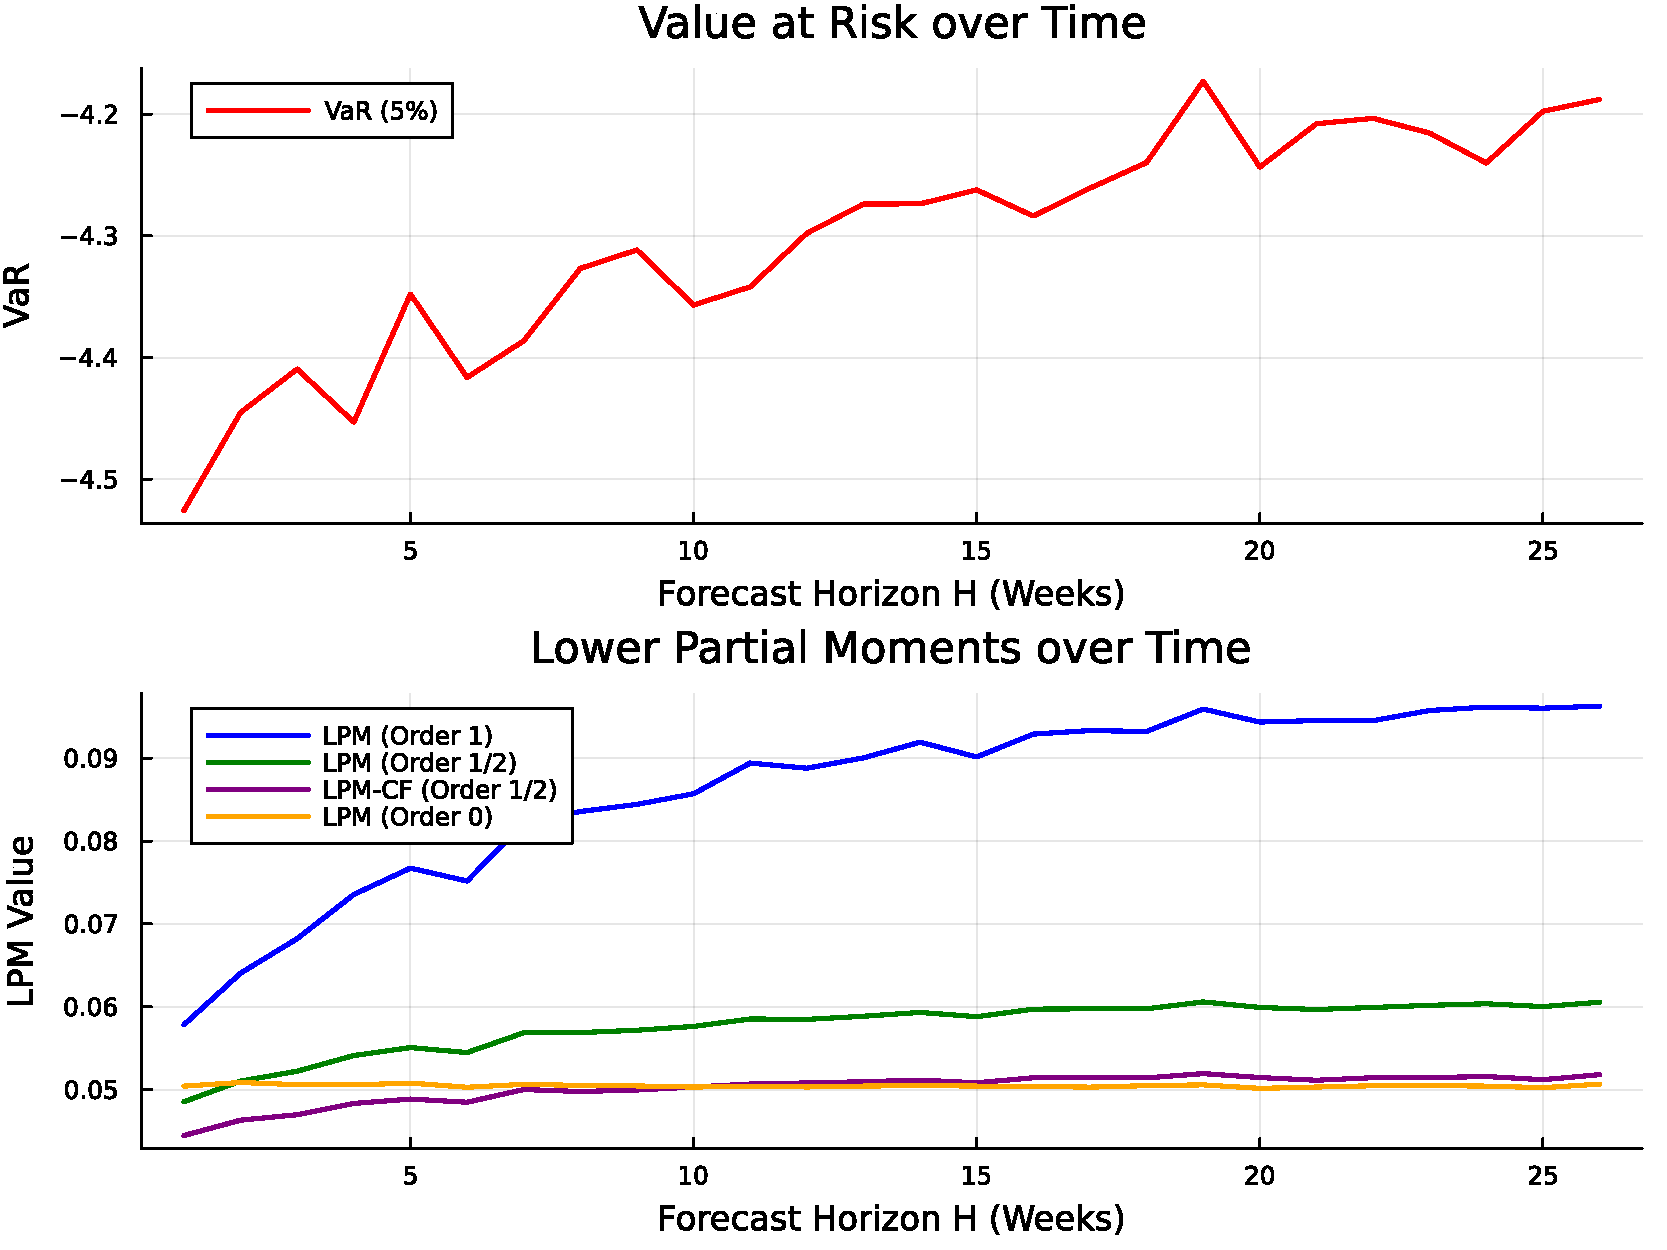
\includegraphics[width=1.0\textwidth]{figures/var_vs_lpm_alternative.pdf}
    \caption{Comparison of VaR and LPM for various orders of LPM}
    \label{fig:var_vs_lpm}
\end{figure}
\begin{itemize}
    \item From figure \ref{fig:var_vs_lpm} we observe that as \(H\) increases, the VaR quantile decreases in absolute magnitude, indicating that extreme losses become less severe relative to shorter horizons. This might seem counterintuitive at first, as stock returns may seem less predictable over larger periods of time, however this observation actually aligns theoretical expectations. That is \(\lim_{h \to \infty} \sigma^2_T(h) = \omega /(1 - \alpha - \beta)\). So as \(H\) increases, \(\sigma^2_T(h)\) will get closer to its unconditional variance and the function will become less steep.
\item As \(H\) increases, \(LPM_1(\tau)\) tends to increase slightly. This suggests that, while the expected downside loss below the threshold \(\tau\) may slightly increase over time, it does so at a decreasing rate. The flattening of the \(LPM_1(\tau)\) function reflects the convergence of the aforementioned unconditional variance which is in line with the theory of GARCH models.
\item As \(H\) increases, \(LPM_0(\tau)\) seems to follow the same trends as the other orders of \(LPM_n(\tau)\). The latter suggests that the downside risk grows marginally as time increases but eventually becomes constant. This is in line with the fact that return distributions converge to their long-run unconditional distribution as time increases.
\item \(LPM_{0.5}(\tau)\) seems to show a gradual increase, as \(H\) increases, after which it eventually flattens. This implies that the frequency and magnitude of downside deviations slowly grow over time and eventually reaching a maximum. The latter reflects the diminishing risk over long periods.
\item As concluded before, fractional moments computed by the Caputo-Fabrizio MGF, inaccurately underestimated. All values of \(LPM_{0.5}(\tau)\) computed via the Caputo-Fabrizio MGF are consistently lower than those computed using direct integration, once more conforming its systematic underestimation of downside risk. The Caputo-Fabrizio MGF approach does not fully capture the tail behaviour of the return distribution, especially for small values \(H\) where it even obtains smaller values compared to \(LPM_0(\tau)\).
\end{itemize}

\subsubsection{Modelling volatility using an observation-driven regression model}
In this final section, we try forecasting volatility using a different model. Namely, we consider an observation-driven regression model, a special case of the Generalized Autoregressive Score framework \cite{creal2013}.
This model has observation equation:
\begin{equation}
    y_t = \beta_t \cdot x_t + \epsilon_t
\end{equation}  
where \(\epsilon_t \sim \mathcal{N}(0, \sigma^2)\) and updating equation:

\begin{equation}
    \beta_t = \omega + \phi \cdot \beta_{t-1} + \alpha(y_{t-1} - \beta_{t-1}\cdot x_{t-1})x_{t-1}
\end{equation}
 This model has the advantage of allowing \(\beta_t\) to evolve over time, in contrast to models like GARCH(1,1) which impose a constant parameter structure. Such time-varying parameters are especially useful when working with financial return series that contain extreme values or structural changes. A fixed parameter may be overly influenced by outliers, whereas a dynamic \(\beta_t\) allows the model to adapt flexibly to such deviations without negatively affecting prediction accuracy. In our application, we let \(y_t\) represent the variance from one-month future returns. We will consider two different versions of the model.
\begin{itemize}
    \item Standard model: we let \(x_t = |r_t|\) represent the absolute return at time \(t\), as in \cite{taylor2007}.
    \item Extended model: we let \(x_t\) represent the conditional expectation of the absolute variance over two weeks of order 0.5. That is \(x_t = \mathbb{E}[|X_{T + 2}|^{0.5} \mid \mathcal{F}_t]\), with \(X_{T + 2}\) defined as before. This choice is motivated by section \ref{sssec:conditional_fractional_moments} where this value was interpreted as the standard deviation of the absolute returns over a period of two weeks.  
\end{itemize}
The goal of this specific case study is to compare the regression performance between a model with and without a moment of fractional order serving as regressor. In order to make sure we focus on this objective and do not get lost in an array of different definitions of fractional moments, we will only consider the fractional moments computed using the expression of the accurate MGFs. It is safe to say that comparing this fractional MGF with the standard model is a lot more useful than comparing a faulty MGF with the standard model.

The dataset has been split as follows: 80\% of the data has been used for the training-set and the remaining 20\% functions as the test-set. Around 50\% of the training-set has been reserved for estimating the parameters of the GARCH(1,1) model. We already estimated the parameters of a GARCH(1,1) model, but the estimates of those parameters were based on the entire dataset. In this case, we need parameter estimates for each different time \(t\) to obtain the most accurate computations of \(\mathbb{E}[|X_{T + 2}|^{0.5} \mid \mathcal{F}_t]\). We still make use of the parameters we estimated in \ref{tab:parameter_estimates} as we let \(\sigma^2_0 = \hat{\omega} / ( 1 - \hat{\alpha} - \hat{\beta})\) be the initial value of \(\sigma^2_t\). We compute \(\mathbb{E}[|X_{T + 2}|^{0.5} \mid \mathcal{F}_t]\) for all \(t\)-values in our selected window. The computation is rather similar to those of section \ref{sssec:conditional_fractional_moments}, with only a slight modification in the code (see algorithm \ref{alg:compute_z}).
After performing Maximum Likelihood Estimation, we obtain the following estimates:
\begin{table}[H]
    \centering
\begin{tabular}{ccccc}
  \toprule
  \textbf{Model} & \textbf{\(\hat{\omega}\)} & \textbf{\(\hat{\phi}\)} & \textbf{\(\hat{\alpha}\)} & \textbf{\(\hat{\sigma^2}\)} \\\midrule
  Standard model & 0.066 & 0.78 & 0.007 & 0.839 \\
  Extended model & 0.08 & 0.812 & 0.219 & 0.683 \\\bottomrule
\end{tabular}

\caption{Parameter Estimates of the two different regression models} 
\label{tab:observation_model}
\end{table}
The two models yield similar estimates for \(\omega\) and \(\phi\). 
The most notable differences appear in the parameter estimates of \(\hat{\alpha}\) and \(\hat{\sigma^2}\). The higher value of  \(\hat{\alpha}\) implies that the updates to \(\beta_t\) of the extended model are more responsive to the product of the past error term and regressor compared to the standard model, namely \(\epsilon_{t -1} \cdot x_{t-1}\). Meanwhile, the smaller value in the extended model \(\hat{\sigma^2}\) of \(\epsilon_{t-1} \sim \mathcal{N}(0, 0.683)\) compared to \(\epsilon_{t-1} \sim \mathcal{N}(0, 0.839)\) indicates reduced variance in the residuals, suggesting a better fit of the model. 

The following plot displays the path of \(\beta_t\) for the standard and extended model, that is, it shows the evolution of the value of \(\beta_t\) over the training period (2010-2022).

\begin{figure}[H]
    \centering
    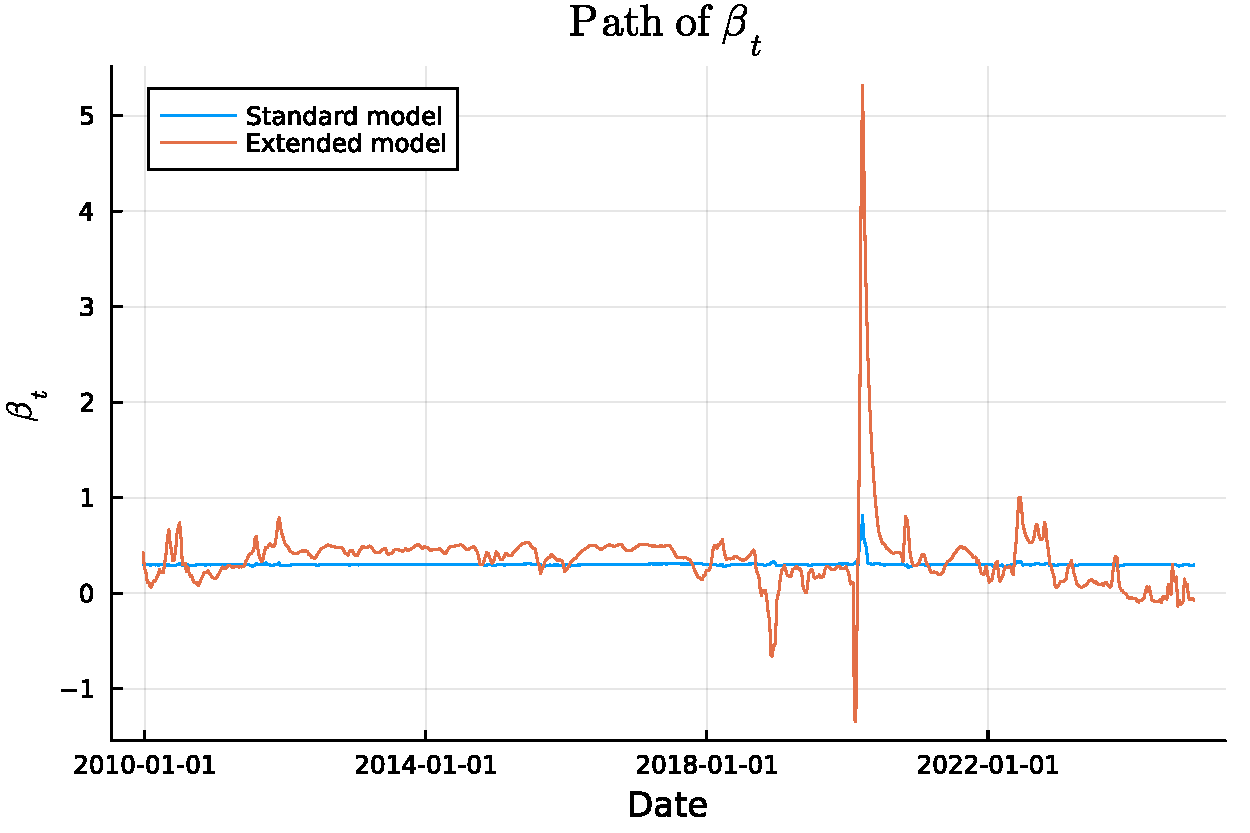
\includegraphics[width=0.7\textwidth]{figures/beta_path_alternative.pdf}
    \caption{Path of \(\beta\) for different models}
    \label{fig:beta_path}
\end{figure}
In the standard model \(\beta_t\) remains relatively stable, clustering around a value of 0.5, except for a spike around 2020 (COVID pandemic). In contrast, the extended model produces a more volatile \(\beta_t\) fluctuating between values around -1 and 5. This is possibly due to how \(\beta_t\) is updated in the extended model. Namely \(\beta_{T + 2}\) is dependent on \(\mathbb{E}[|X_{T + 1}|^{0.5} \mid \mathcal{F}_t]\). We have seen in section \ref{sssec:conditional_fractional_moments} how large these fractional moments can get. Therefore, as the value of \(\mathbb{E}[|X_{T + 1}|^{0.5} \mid \mathcal{F}_t]\) explodes, so will the value \(\beta_t\). The spike during the COVID pandemic perfectly illustrates this behaviour, where greater uncertainty drove up the value of the fractional moment and thus the value of \(\beta_t\).

The table below includes some performance measures of the standard model and extended model respectively.
\begin{table}[H]
    \centering
\begin{tabular}{ccccc}
  \toprule
  \textbf{Model} & \textbf{MSE} & \textbf{MAE} & \textbf{RMSE} & \textbf{\(R^2\)} \\\midrule
  Standard model & 0.275 & 0.387 & 0.524 & 0.023 \\
  Extended model & 0.207 & 0.349 & 0.454 & 0.267 \\\bottomrule
\end{tabular}

\caption{Performance measures of the two different regression models} 
\label{tab:performance_measures}
\end{table}
The values of the mean squared error, mean absolute error and root mean squared error of the extended model are all smaller compared to those of the standard model, indicating that the extended model is preferred. It also achieves a higher value for \(R^2\). Note that \(R^2\) is not always a reliable performance measure for time series data. This follows from the fact that in a time series context, there exists autocorrelation between the residuals, thus violating the assumption that residuals should be independent of each other. Using \(R^2\) in context of time series often results in low values of \(R^2\) indicating poor predictive performance, while this may not necessarily be the case. Yet, in table \ref{tab:performance_measures} we observe that the associated \(R^2\) value of the extended model is roughly ten times the value of the associated \(R^2\) value of the basic model. This suggests that the regressor \(x_t\) in the extended model has a much greater correlation with the variation in \(y_t\) compared to the regressor \(x_t\) in the standard model. That is, the regressor \(x_t\) in the extended model explains a greater portion of the variance in \(y_t\). Thus, in this context, the performance measure \(R^2\) is still found to be useful.
The following figure depicts the actual variance along with the variance predicted by the two different models:

\begin{figure}[H]
    \centering
    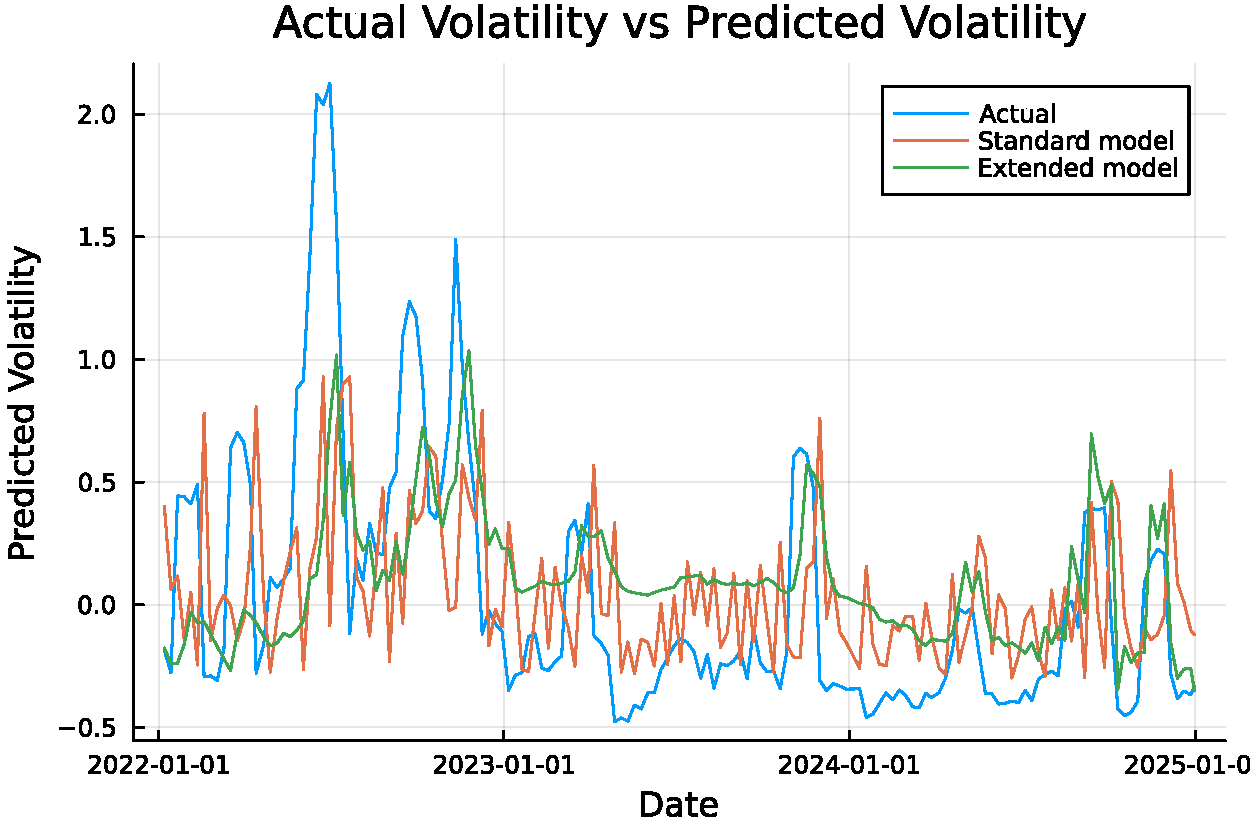
\includegraphics[width=0.7\textwidth]{figures/predicting_volatility.pdf}
    \caption{Actual volatility vs Predicted volatility}
    \label{fig:predicting_volatility}
\end{figure}
From figure \ref{fig:predicting_volatility} we observe that the actual variance attains more extreme values compared to the predictions. While the \(\beta_t\) value of the extended model was more flexible, as shown in figure \ref{fig:beta_path}, it is the predicted volatility of the standard model that fluctuates relatively more. The predicted volatility path of the extended model is much smoother, similar to the actual variances. This might explain the significant difference in performance measures between the two models. 

In conclusion, incorporating an expression involving fractional moments as a regressor leads to an improved performance in predictions of volatility. The extended model not only obtains lower prediction errors, but also better captures the structure of the data. This comes with an increase in volatility of the coefficient path, which may be either an advantage or disadvantage depending on the specific application. 